The flowchart in Figure~\ref{fig:man-inv_tool_workflow} shows the workflow of 
the \invt. Note that orange parts could be used almost out of the 
box, whereas blue parts needed significant extension. Green parts are 
completely implemented from scratch.

\begin{figure}[!ht]
  \centering
  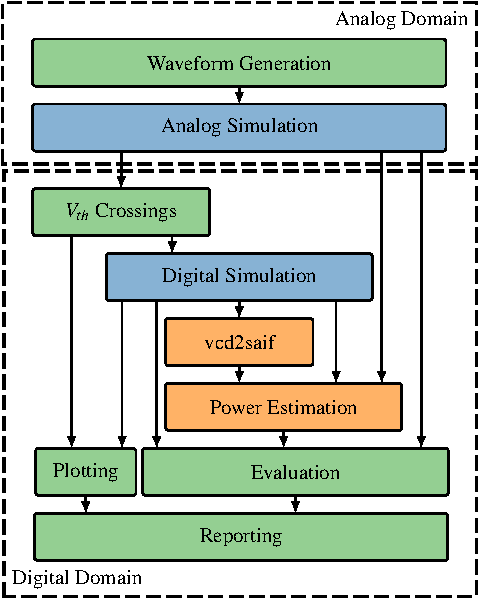
\includegraphics[width=0.75\textwidth]{figures/workflow.pdf}
  \caption{The workflow of the \invt.}
  \label{fig:man-inv_tool_workflow} % \label has to be placed AFTER \caption (or \subcaption) to produce correct cross-references.
\end{figure}

The \invt\ is split into several parts, each part builds upon
the previous parts. The flowchart shows the main steps for a simulation.
Each of the parts corresponds to one or more Makefile recipes.

\subsubsection{Prerequisites}
\label{sec:man-work-prerequisites}

Before the toolchain of the \invt\ can be used, the tool needs a \spice\ / 
\verilog\ description of the circuit and the timing file (\sdffile) for the 
circuit. These files can be generated using for example Cadence Encounter. More 
information on how to prepare a new circuit in 
Section~\ref{sec:man-howto-circuit}.

\subsubsection{Waveform Generation}
\label{sec:man-work-waveform-generation}

Makefile recipes: \emph{generate}

Responsible for generating a new input waveform, according to the
configuration in the directory of the simulated circuit. More
information on the configuration can be found in Section~\ref{sec:man-configuration-waveform}. This section also prepares the
\spfile\ file by replacing placeholders and inserting the generated waveform. 
This 
file is later used by \hspice, \spectre\ or any other \spice\ simulation tool.

\subsubsection{Analog Simulation}
\label{sec:man-work-waveform-analog-simulation}

Makefile recipes: \emph{spice}

Uses the previously generated \spfile\ file and runs the simulation with the 
specified \spice\ simulation tool. The tool can be specified in the 
\configcfgnm{xx} file by setting the variable 
\lstinline|ANALOG_SIMULATION_TOOL| to \lstinline|SPECTRE| or 
\lstinline|HSPICE|. These are currently the tools that are supported by the 
toolchain. Of course, the variables can also be set in the circuit specific 
\configcfg\ file as well, but the default is that \hspice\ is used for 
\SI{65}{\nm} and \spectre\ is used for \SI{15}{\nm}.

\subsubsection{Crossings}
\label{sec:man-work-waveform-crossings}

Makefile recipes: \emph{crossings}

The result of this step is a \crossingsjson\ file, which contains the extracted 
and digitized information of the \spice\ simulation. Depending on the used tool 
in the previous step, the following tasks are performed:
\begin{itemize}
	\item \hspice: The resulting \trfile\ file is parsed and digitized. This is 
	rather time-consuming, since this trace files can get very large. For 
	future releases, parsing the \trfile\ should be replaced with converting 
	the value-change-dump (\vcdfile) file. This is more efficient, since the 
	required data is already digitized, and therefore the file size is reduced.
	\item \spectre: The digitized version of the trace is already generated in 
	the previous step, by extracting the trace from binary trace file 
	(\rawfile). 
	In this step, the resulting \jsonfile\ file is only copied into the 
	crossings 
	folder.
\end{itemize}

\subsubsection{ModelSim}
\label{sec:man-work-waveform-modelsim}

Makefile recipes: \emph{read, gates, sim}

Based on the \crossingsjson\ file, vector files are generated for each input, 
which are later applied to the circuit through the testbench. Since simple 
gates can automatically be generated (see 
Section~\ref{sec:man-configuration-gate}), these gates also need to be created 
before the \modelsim\ simulation starts. The actual simulation uses
\dofile\ files which have been prepared in previous steps, and generate
\vcdfile\ files.

\subsubsection{Power Estimation}
\label{sec:man-work-waveform-power-estimation}

Makefile recipes: \emph{power (power\_spice, power\_dc, power\_pt)}

The power estimation is currently done by two tools: \dc\ (DC) and \primetime\ 
(PT). DC only supports an \emph{average-based} mode, and needs a switching 
activity file (\saiffile) file, which is generated from the value change dump 
(\vcdfile) file from the \modelsim\ simulation. It reduces the information from 
the \vcdfile\ file to a minimum. PT also supports another mode, the so called 
\emph{time-based} mode, which uses more information than the average-based 
mode, because it also considers when the transitions are occurring. Therefore, 
the time-based mode can also estimate the peak power, and not only the average 
power.

\subsubsection{Reporting}
\label{sec:man-work-waveform-reporting}

Makefile recipes: \emph{report}

Since the reporting process is highly customizeable, a shell script is
called for generating the report. This script can be easily adapted by
the user. By default, the script first extracts information from the
various result files of the used tools. The goal is to save this
information in a unified format. The resulting format is a dictionary
that is json serialized and stored into a file called
\resultsjson

Another step in the script is to generate different figures, displaying
the traces of the different delay channel types (\modelsim, Involution)
and the reference trace from \spice. This step also calculates the
deviation between the \spice\ trace (\crossingsjson) and the different
simulations and generates plots for the deviation. After generating the
deviation traces, the tool also calculates the number of glitches and
stores it together with further information about the deviation into a
\csvfile\ file.

Sections where the output is configuration dependent (length of table,
repeating structure with different data) are generated in a further
step. In this step, template files are used so that the user can for
example configure how one row of a table should look like. These
template is used for each row and all resulting rows are finally put together.

The final result of the reporting step is a folder containing all the
required \texfile\ files, the extracted information (\resultsjson),
the generated plots and the \csvfile\ files containing the information about
the deviation. The folder also contains the random waveform that has
been used for simulation, so that the results can be reproduced if
necessary.

